\clearpage
\section{Preliminaries}\label{sec:prel}

This section introduces notation and other preliminaries used in the remainder
of the specification.

\subsection{Notation}

The specification uses set-notation based approach while also inspired
by~\cite{eutxo-2}~and~\cite{eutxo}. Values $a$ are in a set $a \in \mathcal{A}$,
also indicated as being of some type $a : \mathcal{A}$, and multidimensional values are
tuples drawn from a $\times$ product of multiple sets, e.g.
$(a,b) \in (\mathcal{A} \times \mathcal{B})$. An empty set is indicated by
$\emptyset$ and sets may be enumerated using $\{a_1 \dots a_n\}$ notation. The $=$ operator means
equality and $\gets$ is explicit assignment of a variable or value to one
or more variables. Projection is used to access the elements of a tuple, e.g.
${(a,b)}^{\downarrow1} = a$. Functions are morphisms mapping from one set to another
$x : \mathcal{A} \to f(x) : \mathcal{B}$, where function
application of a function $f$ to an argument $x$ is written as $f(x)$. \\

\noindent Furthermore, given a set $\mathcal{A}$, let
\begin{itemize}
	\item $\mathcal{A}^? = \mathcal{A} \cup \Diamond$ denotes an option: a value from $\mathcal{A}$ or no value at all indicated by $\bot$,
	\item $\mathcal{A}^n$ be the set of all n-sized sequences over $\mathcal{A}$,
	\item $\mathcal{A}^! = \bigcup_{i=1}^{n \in \tyNatural} \mathcal{A}^{i}$ be the set of non-empty sequences over $\mathcal{A}$, and
	\item $\mathcal{A}^* = \bigcup_{i=0}^{n \in \tyNatural} \mathcal{A}^{i}$ be
	      the set of all sequences over $\mathcal{A}$.
\end{itemize}

\noindent With this, we further define:
\begin{itemize}
	\item $\tyBool = \{\false, \true\}$ are boolean values
	\item $\tyNatural$ are natural numbers $\{0, 1, 2, \ldots\}$
	\item $\tyInteger$ are integer numbers $\{\ldots, -2, -1, 0, 1, 2, \ldots\}$
	\item $\tyBytes = \bigcup_{n=0}^{\inf}{\{0,1\}}^{8n}$ denotes a arbitrary
	      string of bytes
	\item $\concat : \tyBytes^* \to \tyBytes$ is concatenating bytes, we also use operator $\bigoplus$ for this
	\item $\hash : x \to \tyBytes$ denotes a collision-resistant
	      hashing function and $x^{\#}$ indicates the hash of $x$
	\item $\bytes : x \to \tyBytes$ denotes an invertible serialisation function
	      mapping arbitrary data to bytes
	\item $a || b = \concat(\bytes(a), \bytes(b))$ is an operator which concatenates the $\bytes(b)$ to the $\bytes(a)$
	\item Lists of values $l \in \mathcal{A}^{*}$ are written as
	      $l = [x_{1}, \ldots, x_{n}]$. Empty lists are denoted by $[]$, the $i$th
	      element $x_{i}$ is also written $l[i]$ and the length of the list is
	      $|l| = n$. An underscore is also used to indicate a list of values
	      $\underline{x} = l$. Projection on lists are mapped to their elements,
	      i.e.
	      $\underline{x}^{\downarrow1} = [x_{1}^{\downarrow1}, \dots, x_{n}^{\downarrow1}]$.
	\item $\sortOn : i \to \mathcal{A}^{*} \to \mathcal{A}^{*}$ does sort a list of
	      values on the $i$th projection.
	\item $\tyData$ is a universal data type of nested sums and products built up
	      recursively from the base types of $\tyInteger$ and $\tyBytes$.
\end{itemize}

\subsection{Public key multi-signature scheme}\label{sec:multisig}
% TODO: move/merge with protocol setup and make concrete
\noindent A multisignature scheme is a set of algorithms where
\begin{itemize}
	\item $\msSetup$ generates public parameters $\msParams$, such that
	\item $(\msVK,\msSK) \gets \msKeyGen(\msParams)$ can be used to generate fresh
	      key pairs,
	\item $\msSig \gets \msSign(\msParams,\msSK,\msMsg)$ signs a message $\msMsg$
	      using key $\msSK$,
	\item $\msCVK \gets \msCombVK(\msParams,\msVKL)$ aggregates a list of
	      verification keys $\msVKL$ into a single, aggregate key $\msCVK$,
	\item $\msCSig \gets \msComb(\msParams,\msMsg,\msVKL,\msSigL)$ aggregates a
	      list of signatures $\msSigL$ about message $m$ into a single, aggregate
	      signature~$\msCSig$.
	\item $\msVfy(\msParams,\msCVK,\msMsg,\msCSig) \in \tyBool$ verifies an aggregate
	      signature $\msCSig$ of message $\msMsg$ under an aggregate verification
	      key $\msCVK$.
\end{itemize}

The security definition of a multisignature scheme
from~\cite{itakura1983public,CCS:MicOhtRey01} guarantees that, if $\msCVK$ is
produced from a tuple of verification keys $\msVKL$ via $\msCombVK$, then no
aggregate signature $\msCSig$ can pass verification
$\msVfy(\msCVK,\msMsg,\msCSig)$ unless all honest parties holding keys in
$\msVKL$ signed $m$.

Note that in the following, we make the parameter~$\msParams$ implicit and leave
out the $ver$ suffix for verification key such that $k = k^{ver}$ for better
readability.

\subsection{Extended UTxO}\label{sec:eutxo}
The Hydra Head protocol is specified to work on the so-called Extended UTxO (EUTxO) ledgers
like Cardano.

The basis for EUTxO is Bitcoin's UTxO ledger
model~\cite{formal-model-of-bitcoin-transactions,Zahnentferner18-UTxO}.
Intuitively, it arranges transactions in a directed acyclic graph, such as the
one in Figure~\ref{fig:utxo-graph}, where boxes represent transactions with
(red) inputs to the left and (black) outputs to the right. A dangling
(unconnected) output is an \emph{unspent transaction output (UTxO)} --- there
are two UTxOs in the figure.

\begin{figure}[h]
	\centering
        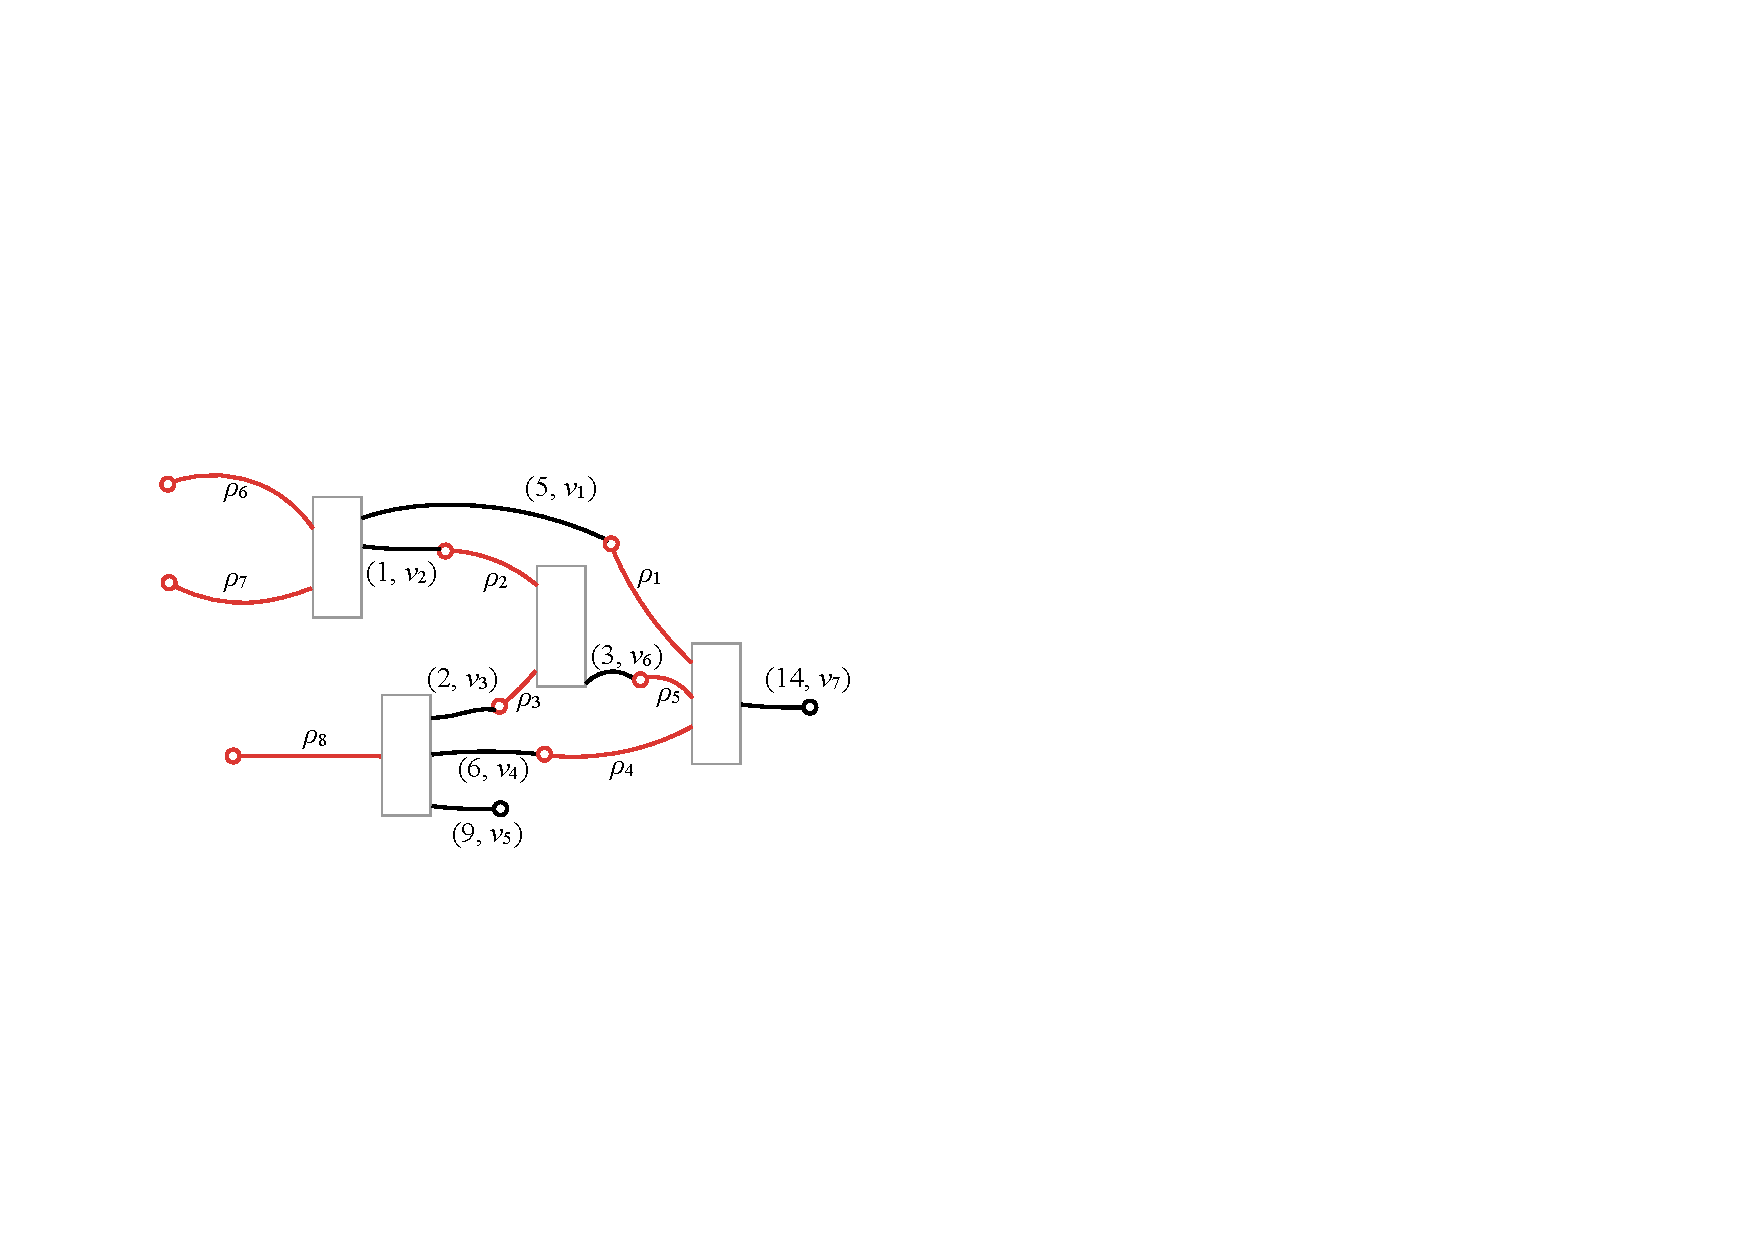
\includegraphics[width=0.5\textwidth]{Hydra/Protocol/Figures/utxo-graph.pdf}
	\caption{Example of a plain UTxO graph}\label{fig:utxo-graph}
\end{figure}

The following paragraphs will give definitions of the UTxO model and it's
extension to support scripting (EUTxO) suitable for this Hydra Head protocol
specification. For a more detailed introduction to the EUTxO ledger model,
see~\cite{eutxo},~\cite{eutxo-2}~and~\cite{utxo-ma}.

\subsubsection{Values}

\begin{definition}[Values]
	Values are sets that keep track of how many units of which tokens of which
	currency are available. Given a finitely supported function $\mapsto$, that
	maps keys to monoids, a value is the set of such mappings over currencies
	(minting policy identifiers), over a mapping of token names $t$ to
	quantities $q$:
	\[
		\val \in \tyValue = (c : \tyBytes \mapsto (t : \tyBytes \mapsto q : \tyInteger))
	\]
	\noindent where addition of values is defined as $+$ and $\varnothing$ is the empty value.
\end{definition}

For example, the value $\{c_{1} \mapsto \{t_1 \mapsto 1, t_2 \mapsto 1\}\}$
contains tokens $t_1$ and $t_2$ of currency $c_{1}$ and addition merges
currencies and token names naturally:
\begin{align*}
	     & \{c_{1} \mapsto \{t_1 \mapsto 1, t_2 \mapsto 1\}\}                                                        \\
	+ \  & \{c_{1} \mapsto \{t_{2} \mapsto 1, t_3 \mapsto 1\}, c_{2} \mapsto \{ t_{1} \mapsto 2\}\}                  \\
	= \  & \{c_{1} \mapsto \{t_1 \mapsto 1, t_2 \mapsto 2, t_3 \mapsto 1\}, c_{2} \mapsto \{ t_{1} \mapsto 2\}\} \ .
\end{align*}

While the above definition should be sufficient for the purpose of this
specification, a full definition for finitely supported functions and values as
used here can be found in~\cite{utxo-ma}. To further improve readability, we
define the following shorthands:
\begin{itemize}
	\item $\{t_1, \ldots, t_n\} :: c$ for a set positive single quantity assets
	      $\{c \mapsto \{t_1 \mapsto 1, \ldots, t_n \mapsto 1\}\}$,
	\item ${\{t_1, \ldots, t_n\}}^{-1} :: c$ for a set of negative single quantity assets
	      $\{c \mapsto \{t_1 \mapsto -1, \ldots, t_n \mapsto -1\}\}$,

	\item $\{c \mapsto t \mapsto q\}$ for the value entry $\{c \mapsto \{t \mapsto q\}\}$,
	\item $\{c \mapsto \cdot \mapsto q \}$ for any asset with currency $c$ and
	      quantity $q$ irrespective of token name.
\end{itemize}

\subsubsection{Scripts}

Validator scripts are called \emph{phase-2} scripts in the Cardano Ledger
specification (see~\cite{ledger-alonzo-spec} for a formal treatment of these). Scripts
are used for multiple purposes, but most often (and sufficient for this
specification) as a \emph{spending} or \emph{minting} policy script.

\begin{definition}[Minting Policy Script]
	A script $\mu \in \mathcal{M}$ governing whether a value can be minted (or
	burned), is a pure function with type
	\[
		\mu \in \mathcal{M} = (\rho : \tyData) \to (\txContext : \tyContext) \to\tyBool,
	\]
	where $\rho \in \tyData$ is the redeemer provided as part of the transaction
	being validated and $\txContext \in \tyContext$ is the validation
	context.
\end{definition}

\begin{definition}[Spending Validator Script]
	A validator script $\nu \in \mathcal{V}$ governing whether an output can be
	spent, is a pure function with type
	\[
		\nu \in \mathcal{V} = (\delta : \tyData) \to (\rho : \tyData) \to (\txContext : \tyContext) \to\tyBool,
	\]
	where $\delta \in \tyData$ is the datum available at the output to be spent,
	$\rho \in \tyData$ is the redeemer data provided as part of the transaction
	being validated, and $\txContext \in \tyContext$ is the validation
	context.
\end{definition}

\subsubsection{Transactions}
\todo{actual transactions $\mathcal{T}$ are not defined}

We define EUTxO inputs, outputs and transactions as they are available to
scripts and just enough to specify the behavior of the Hydra validator scripts.
For example outputs addresses and datums are much more complicated in the full
ledger model~\cite{eutxo-2, ledger-shelley-spec}.

\begin{definition}[Outputs]
	An output $o \in \txOutputs$ stores some value $\val \in \tyValue$ at some address,
	defined by the hash of a validator script $\nu^{\#} \in \tyBytes = \hash(\nu \in \mathcal{V})$,
	and may store (reference) some data $\delta \in \tyData$:
	\[
		o \in \txOutputs = (\val : \tyValue \times \nu^{\#} : \tyBytes \times \delta : \tyData)
	\]
\end{definition}

\begin{definition}[Output references]
	An output reference $\txOutRef \in \tyOutRef$ points to an output of a
	transaction, using a transaction id (that is, a hash of the transaction body)
	and the output index within that transaction.
	\[
		\txOutRef \in \tyOutRef = (\tyBytes \times \mathbb{N})
	\]
\end{definition}

\begin{definition}[Inputs]
	A transaction input $i \in \txInputs$ is an output reference
	$\txOutRef \in \tyOutRef$ with a corresponding redeemer $\rho \in \tyData$:
	\[
		i \in \txInputs = (\txOutRef : \tyOutRef \times \rho : \tyData)
	\]
\end{definition}

\begin{definition}[Validation Context]
	A validation context $\txContext \in \tyContext$ is a view on the transaction
	to be validated:
	\[
		\txContext \in \tyContext = (\tyInputs \times \tyOutputs \times \tyValue \times \mathcal{S}^{\leftrightarrow} \times \mathcal{K})
	\]
	where $\txInputs \in \tyInputs$ is a \textbf{set} of inputs,
	$\txOutputs \in \tyOutputs$ is a \textbf{list} of outputs,
	$\txMint \in \tyValue$ is the minted (or burned) value,
	$(\txValidityMin, \txValidityMax) \in \tyValidity$ are the lower and upper
	validity bounds where $\txValidityMin <= \txValidityMax$, and
	$\txKeys \in \mathcal{K}$ is the set of verification keys which signed the
	transaction.
	% TODO: \tyValidity undefined, define time, periods and intervals?
\end{definition}

Informally, scripts are evaluated by the ledger when it applies a transaction to
its current state to yield a new ledger state (besides checking the transaction
integrity, signatures and ledger rules). Each validator script referenced by
an output is passed its arguments drawn from the output it locks and the
transaction context it is executed in. The transaction is valid if and only if
all scripts validate, i.e. $\mu(\rho, \txContext) = \true$ and
$\nu(\delta, \rho, \txContext) = \true$.

\subsubsection{State machines and graphical notation}

State machines in the EUTxO ledger model are commonly described using the
\emph{constraint emitting machine (CEM)} formalism~\cite{eutxo}, e.g.~the
original paper describes the Hydra Head protocol using this
notation~\cite{hydrahead20}. Although inspired by CEMs, this specification uses
a more direct representation of individual transactions to simplify description
of non-state-machine transactions and help translation to concrete
implementations on Cardano. The structure of the state machine is enforced
on-chain through \emph{scripts} which run as part of the ledger's validation of
a transaction (see Section~\ref{sec:eutxo}). For each protocol transaction, the
specification defines the structure of the transaction and enumerates the
transaction constraints enforced by the scripts ($\cemTxCon$ in the CEM
formalism).

% TODO: Create example, maybe using the collectComTx, but with generic labels
% and point out that state input/outputs do represent a transition in the
% statemachine from s' to s' etc.
\todo{Add an example graph with a legend}

%%% Local Variables:
%%% mode: latex
%%% TeX-master: "main"
%%% End:
